\documentclass{beamer}
% This is the preamble where you can add packages and change global settings.

% You can find many more presentation examples using beamer here: 
% http://www2.informatik.uni-freiburg.de/~frank/ENG/latex-course/latex-course-3/latex-course-3_en.html

% The guts of this beamer presentation were take from example.tex from the above website.

% Look at example 9 for how to make pdf handouts of slides.
\usepackage{verbatim}
%------------------------------------------------------------------------------
\usepackage{xspace}
%------------------------------------------------------------------------------
\usepackage{pdfpages} % this allows us to include our Example!/*.pdf files
%------------------------------------------------------------------------------
\usepackage{syntonly} % just check the syntax, don't actually compile.
%\syntaxonly
%------------------------------------------------------------------------------
\usepackage{amssymb} % AMS symbols like a \checkmark
%------------------------------------------------------------------------------
\usepackage{tikz}
\usetikzlibrary{calc}
\newcommand{\polygon}[2]{%
  let \n{len} = {2*#2*tan(360/(2*#1))} in
 ++(0,-#2) ++(\n{len}/2,0) \foreach \x in {1,...,#1} { -- ++(\x*360/#1:\n{len})}}
%------------------------------------------------------------------------------
\usepackage{hyperref}
\hypersetup{
     colorlinks   = true,
     citecolor    = gray,
     linkcolor    = blue,
     urlcolor     = blue
}
%------------------------------------------------------------------------------
\begin{document}

\newcommand{\latex}{\LaTeX\xspace}
\newcommand{\tex}{\TeX\xspace}

\title{\latex Tutorial}   
\author{Dylan Mikesell} 
\date{30 September 2015} 

\frame{\titlepage} 

\frame{\frametitle{Outline}\tableofcontents} 


\section{\latex: What is it?} 
%------------------------------------------------------------------------------
\frame{\frametitle{\latex} 
\begin{itemize}
	\item \latex is a typesetting package that is used to make high quality documents
	\item It can be used to make scientific and mathematical documents
	\item It can be used to make letters, books, and many other types of documents (e.g. this presentation!)
\end{itemize}

\pause
\latex is available for most computers, from PC to Mac to UNIX 

\vspace{\baselineskip}

We are not here to learn how to install and set up a \latex system, but to
learn how to write a document so that it can be processed by \latex.
}
%------------------------------------------------------------------------------
% Chapter 1 tells you about the basic structure of LATEX 2ε documents. You
% will also learn a bit about the history of LATEX. After reading this
% chapter, you should have a rough understanding how LATEX works.
%------------------------------------------------------------------------------
\frame{\frametitle{\tex} 
	\tex is a computer program created by Donald E. Knuth to typeset text and
	mathematical formulae.
	
	\vspace{\baselineskip}

	\latex enables the author to typeset and print their work at the highest typographical quality, using a predefined, professional layout. 
	
	\vspace{\baselineskip}
	
	\latex uses the \tex formatter as its typesetting engine.
}
%------------------------------------------------------------------------------
\frame{\frametitle{\latex vs. MS Word and OpenOffice}

	Word processors (e.g. MS Word and OpenOffice) are WYSIWYG programs.

	\vspace{\baselineskip}

	\latex is a WYSIWYW program. \latex does the role of formatting and designing the document. (You do not see the final product until you compile the document!)

	\vspace{\baselineskip}

	But \latex is only a program, and the user/author has to provide information about the structure of the document using \latex commands.
}
%------------------------------------------------------------------------------
\frame{\frametitle{So why use \latex?}

	With WYSIWYG systems, authors often generate aesthetically pleasing
	documents with very little or inconsistent structure. 

	\vspace{\baselineskip}

	\latex prevents such formatting errors by forcing the author to declare
	the logical structure of the document. \latex then chooses the most
	suitable layout and use of the page.
}
%------------------------------------------------------------------------------
\frame{\frametitle{}

	\begin{block}{Advantages}
	\begin{itemize}
		\item Complex mathematical formulae are supported in a simple way
		\item Users only need to learn a few basic commands to specify the structure of the document
		\item Complex structures like footnotes, bibliographies, tables of contents, etc. are easily generated
		\item Internal referencing within a document is incredibly easy
		\item Free add-on packages exist (e.g. to typeset a particular bibliography format)
		\item Documents look professional!
	\end{itemize}
	\end{block}

	\begin{block}{Disadvantages}
	\begin{itemize}
		\item Designing a completely new document layout is difficult
		\item The learning curve can be steep for those who do grasp the concept of logical markup right away
	\end{itemize}
	\end{block}
}
%------------------------------------------------------------------------------
% Chapter 2 goes into the details of typesetting your documents. It explains
% most of the essential LATEX commands and environments. After reading this
% chapter, you will be able to write your first documents.
\section{Preliminaries and \latex commands}

\frame{\frametitle{Preliminaries}

	\begin{block}{Whitespace}
	\begin{itemize}
		\item \textit{Whitespace} characters such as blank, tab, or space are treated the same by \latex
		\item \textit{Whitespace} at the start of a line is usually ignored
		\item A single line break is treated as \textit{Whitespace}
		\item An empty line between two lines of text defines a paragraph
		\item Several empty lines are treated the same as \textit{one} empty line
	\end{itemize}
	\end{block}

	\begin{block}{Special characters}
	\begin{itemize}
		\item The following symbols are reserved by \latex and have special meaning:
		\item[] \# \xspace \$ \xspace \% \xspace \^ \xspace \xspace \& \xspace \_ \xspace \{ \xspace \} \xspace \~ \xspace \xspace \textbackslash
	\end{itemize}
	\end{block}
	}
%------------------------------------------------------------------------------
\frame{\frametitle{\latex commands}

	\begin{itemize}
		\item \latex commands are case sensitive
		\item commands start with a \textbackslash \xspace and then have a name consisting of letters only
		\item commands are terminated by a space, a number or any other 'non-letter'
		\item Some commands require a parameter given between \{ \xspace \}
		\item Some commands take optional parameters between [ \xspace ]
		\item[] e.g. {\textbackslash}\textit{command}[\textit{optional parameters}]\{\textit{parameter}\}
		\pause
		\item Many commands exist in a 'starred variant', where the '*' is appended to the command name
		\item[] e.g. {\textbackslash}section*\{Introduction\}
	\end{itemize}
}
%------------------------------------------------------------------------------
\frame{\frametitle{Comments...just like MATLAB}

	\begin{itemize}
		\item \latex comments are indicated by \%
		\item You can also indicate multiple lines of comments by using the \textbf{comment} environment
	\end{itemize}
	e.g.\\
	
	\vspace{\baselineskip}
	
	{\textbackslash}begin\{comment\}\\
		\hspace{0.2cm} Everything written within the environment begin and end is a comment!\\
	{\textbackslash}end\{comment\}
	
	\vspace{\baselineskip}

	or

	\vspace{\baselineskip}
	
	{\textbackslash}includegraphics\{myFigure.pdf\} \% This is also a comment.
}
%------------------------------------------------------------------------------
\section{The \latex input file}
%------------------------------------------------------------------------------
\frame{\frametitle{\latex input file}
	When \latex processes an input file it expects a few commands in a certain order:

	\vspace{\baselineskip}

	\begin{enumerate}
		\item {\textbackslash}documentclass\{\ldots\} \% this specifies the document type
		\item {\textbackslash}usepackage\{\ldots\} \% this adds functionality 
		\item {\textbackslash}begin\{document\} \% start the body of the text
		\item {\textbackslash}end\{document\} \%  end the body of the text; anything after this is ignored by \latex
	\end{enumerate}
}
%------------------------------------------------------------------------------
\begin{frame}[fragile]{A simple example}

	Make a file called myFirstLatex.tex\footnotemark[1] and put the following in the file.

	\vspace{\baselineskip}

	\begin{verbatim}
	\documentclass{article}
	\begin{document}
	This is my first \LaTex document.
	\end{document}
	\end{verbatim}

	Then run the command \textit{pdflatex myFirstLatex.tex} in the command line (or compile this with your preferred \latex IDE.)


	\footnotetext[1]{You can go to \textit{Example1/} in the \textit{Resources/} folder in the git repository to find myFirstLatex.tex.}
\end{frame}

%------------------------------------------------------------------------------
\setbeamercolor{background canvas}{bg=}

\begin{frame}{The output}

	
\includepdf[pages={1},frame=true,scale=0.8]{Example1/myFirstLatex.pdf}

	\pause

	We notice the poor spacing between \latex and document. How can we fix this?
\end{frame}
%------------------------------------------------------------------------------
\begin{frame}[fragile]{Fixing the simple example}

	Make a file called mySecondLatex.tex\footnotemark[1] and put the following in the file.

	\vspace{\baselineskip}

	\begin{verbatim}
	\documentclass{article}
	\usepackage{xspace}
	\begin{document}
	This is my first \LaTex \xspace document.
	\end{document}
	\end{verbatim}

	Then run the command \textit{pdflatex mySecondLatex.tex} in the command line (or compile this with your preferred \latex IDE.)


	\footnotetext[1]{You can go to \textit{Example2} in the \textit{Resources/} folder in the git repository to find mySecondLatex.tex.}
\end{frame}
%------------------------------------------------------------------------------
\begin{frame}{The output}

	
\includepdf[pages={1},frame=true,scale=0.8]{Example2/mySecondLatex.pdf}
	
	\pause

	To see the manual for the \textit{xspace} package type \textit{texdoc xspace} at the command line.	
\end{frame}
%------------------------------------------------------------------------------
\begin{frame}[fragile]{Making your own \latex command}

	Make a file called myThirdLatex.tex\footnotemark[1] and put the following in the file.

	\vspace{\baselineskip}

	\begin{verbatim}
	\documentclass{article}
	\usepackage{xspace}
	\newcommand{\latex}{\LaTeX\xspace}
	\begin{document}
	This is my first \latex document.
	\end{document}
	\end{verbatim}

	Then run the command \textit{pdflatex myThirdLatex.tex} in the command line (or compile this with your preferred \latex IDE.)


	\footnotetext[1]{You can go to \textit{Example3} in the \textit{Resources/} folder in the git repository to find myThirdLatex.tex.}
\end{frame}
%------------------------------------------------------------------------------
\begin{frame}{The output}

	
\includepdf[pages={1},frame=true,scale=0.8]{Example3/myThirdLatex.pdf}
	
\end{frame}
%------------------------------------------------------------------------------
\begin{frame}[fragile]{A complete document}

	Make a file called myFourthLatex.tex\footnotemark[1] and put the following in the file.

	\begin{verbatim}
	\documentclass{article}
	\usepackage{xspace}
	\newcommand{\latex}{\LaTeX\xspace}
	\author{Dylan Mikesell} % define the author
	\title{\latex Tutorial} % define the title
	% end the PREAMBLE
	\begin{document}
	\maketitle % generate the title
	\tableofcontents % make a table of contents
	\section{My first section} % make a section for the table of contents
	% type some words
	This is my first \latex document.
	\section{Adios} % make a final section
	\ldots{} and that's it.
	\end{document}
	\end{verbatim}

\end{frame}
%------------------------------------------------------------------------------
\begin{frame}{The output}

	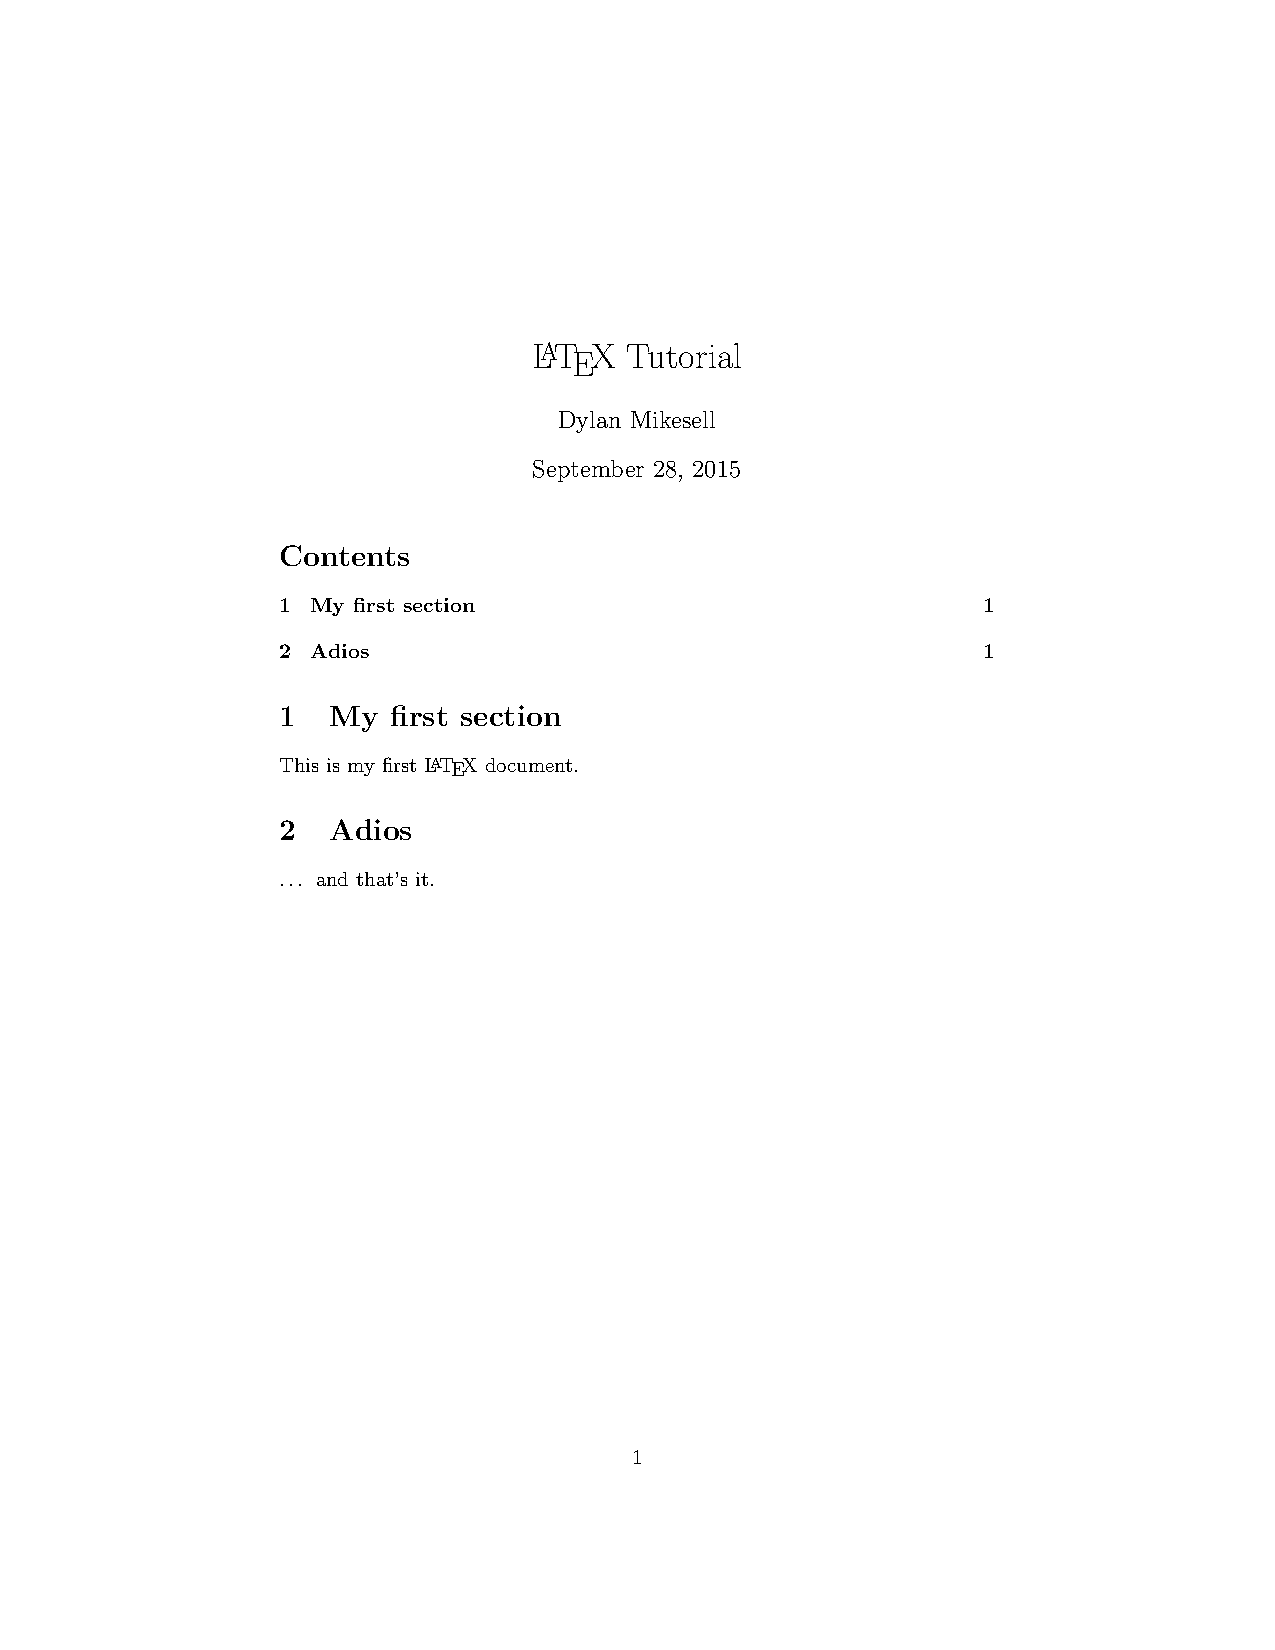
\includepdf[pages={1},frame=true,scale=0.8]{Example4/myFourthLatex.pdf}
	
\end{frame}
%------------------------------------------------------------------------------
\begin{frame}[fragile]{Adding a figure }

	Open the file called myFifthLatex.tex.

	\begin{verbatim}
	\documentclass{article}
	\usepackage{graphicx} % need to include the 'graphicx'
	\graphicspath{{./Figs/}} % Tell LaTeX where it should look 
	for your figures...
	\begin{document}
	\maketitle...
	This is my first \latex document. And this is my first 
	figure reference (Fig.~\ref{fig:firstFigure}).
	\begin{figure}
		\centering
		
\includegraphics[width=0.5\columnwidth]{LaTeXLogo.png}
		\caption{This is my first figure.}
		\label{fig:firstFigure}
	\end{figure}
	\end{verbatim}

	% \footnotetext[1]{You can go to \textit{Example5} in the \textit{Resources/} folder in the git repository to find myFifthLatex.tex.}

\end{frame}
%------------------------------------------------------------------------------
\begin{frame}{The output}

	
\includepdf[pages={3},frame=true,scale=0.8]{Example5/myFifthLatex.pdf}
	
\end{frame}
%------------------------------------------------------------------------------
\begin{frame}[fragile]{Adding a table}

	Open the file called mySixthLatex.tex.

	\begin{verbatim}
	\documentclass{article}
	\usepackage{graphicx} % need to include the 'graphicx'
	\graphicspath{{./Figs/}} % Tell LaTeX where it should look 
	for your figures...
	\begin{document}
	\maketitle...
	This is my first table (Tab.~\ref{tab:firstTable}).
	\begin{table}[b]
		\begin{tabular}{l|c|r}
		$a \approx b$ & $a \ne b$ & $a = \int_{t_0}^{t_1} \frac{g(t)}{t} dt $ \\ \hline
		\textbf{column 1} & \textbf{column 2} & \textbf{column 3} \\ \hline
		\end{tabular}
		\caption{I just made my first table!}
		\label{tab:firstTable}
	\end{table}
	\end{verbatim}


\end{frame}
%------------------------------------------------------------------------------
\begin{frame}{The output}

	
\includepdf[pages={3},frame=true,scale=0.8]{Example6/mySixthLatex.pdf}
	
\end{frame}
%------------------------------------------------------------------------------
\begin{frame}[fragile]{Adding equations}

	Open the file called mySeventhLatex.tex.

	\begin{verbatim}
	$$ a = \frac{1}{N} $$
	
	\begin{equation}
		A\mathbf{x} = \mathbf{y}
		\label{eqn:equation}
	\end{equation}

	\begin{eqnarray}
		\nonumber
		A\mathbf{x} = \mathbf{y} \\
		while \ x_{i} \ge 0 
		\label{eqn:eqnarray}
	\end{eqnarray}
	\end{verbatim}


\end{frame}
%------------------------------------------------------------------------------
\begin{frame}{The output}

	
\includepdf[pages={3},frame=true,scale=0.8]{Example7/mySeventhLatex.pdf}
	
\end{frame}
%------------------------------------------------------------------------------
\begin{frame}{Bibliography}

	
\includepdf[pages={3},frame=true,scale=0.8]{Example8/myEigthLatex.pdf}

	\footnotetext[1]{You can go to \textit{Example8} in the \textit{Resources/} folder in the git repository to find myEightLatex.tex.}
\end{frame}
%------------------------------------------------------------------------------
\begin{frame}{natbib package}

	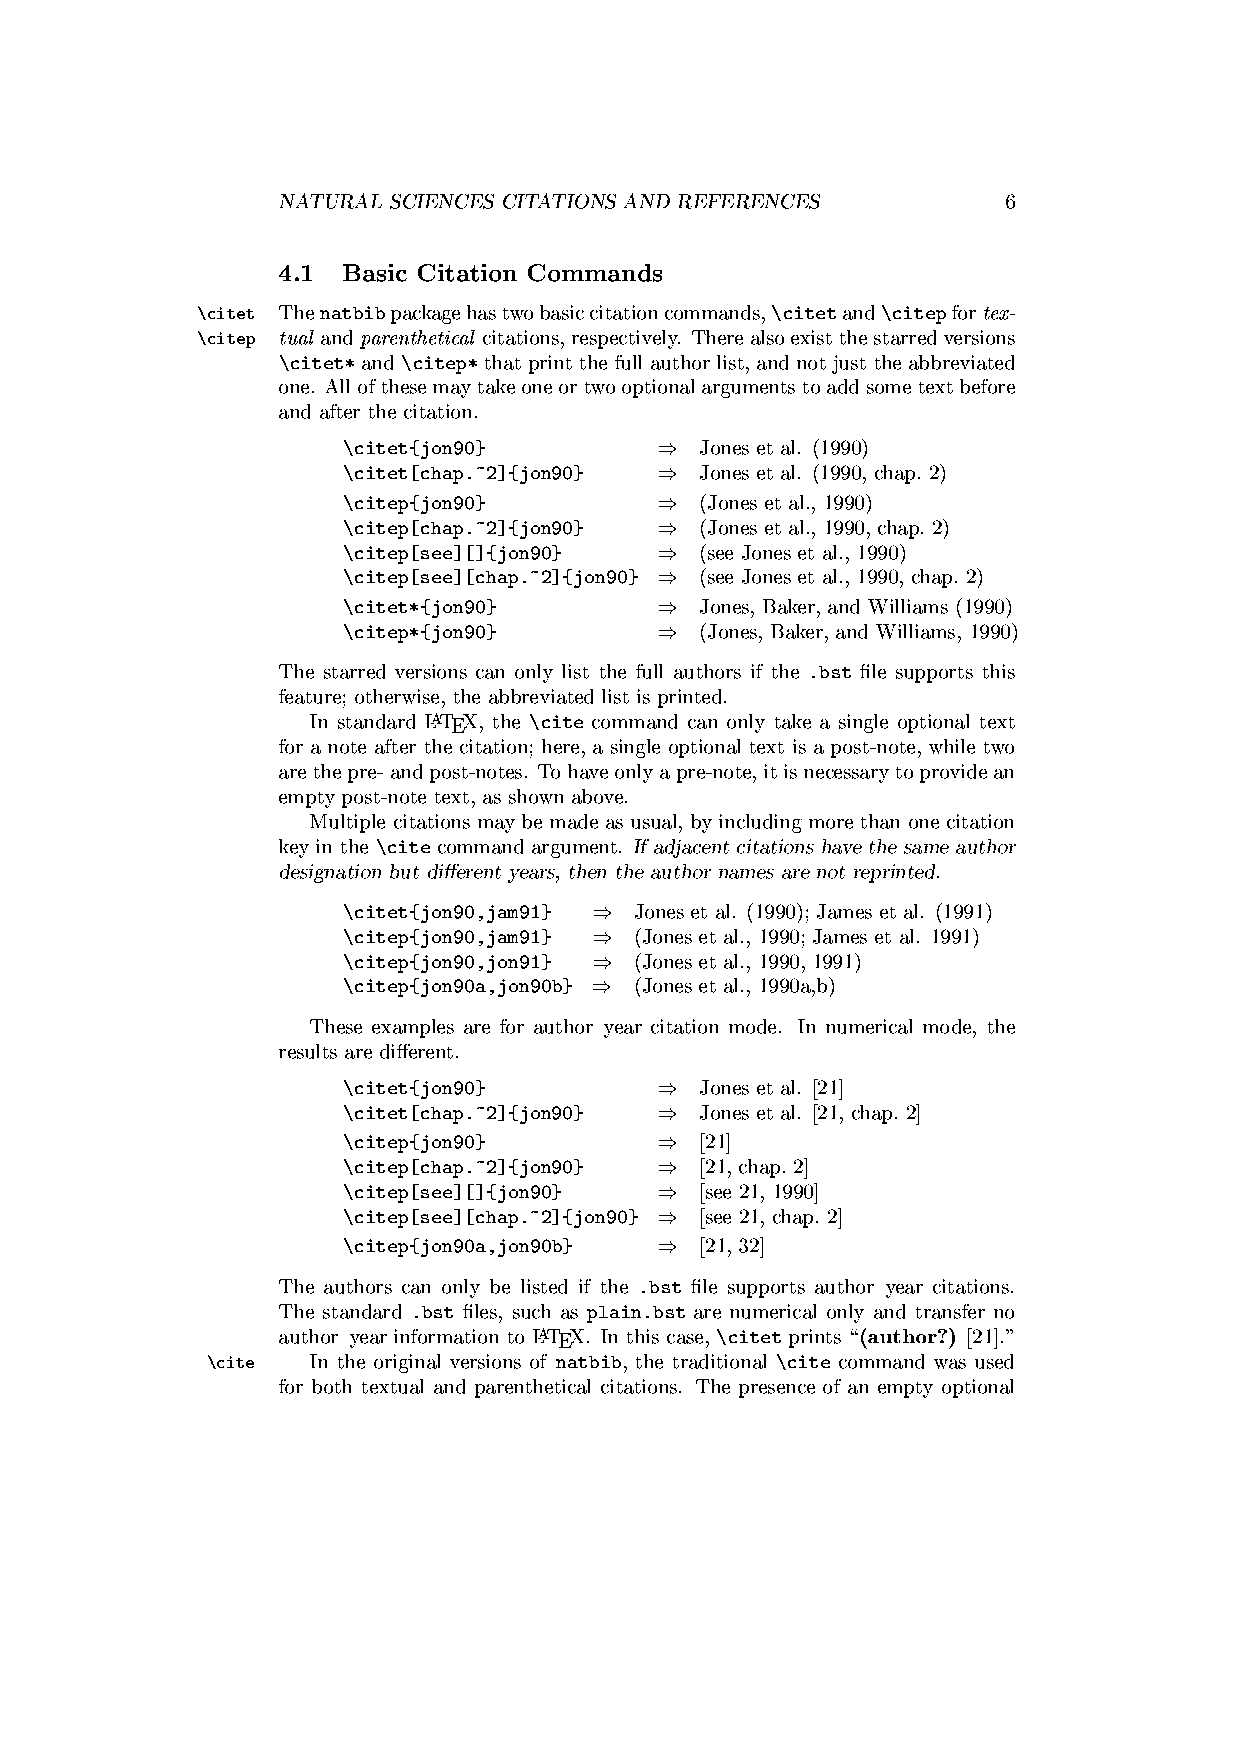
\includepdf[pages={1},frame=true,scale=0.8]{../natbib.pdf}

\end{frame}
%------------------------------------------------------------------------------
\begin{frame}[fragile]{Bulleted list}
	\begin{columns}[c]
		\begin{column}{0.48\textwidth}
			\begin{verbatim}
			\begin{itemize}
				\item This is the default 
					bullet
				\item[X] This is an X bullet
				\item[\checkmark] This is 
					a \checkmark bullet from 
					\usepackage{amssym}
			\end{itemize}
			\end{verbatim}
		\end{column}
		\hfill
		\begin{column}{0.48\textwidth}
			\begin{itemize}
				\item This is the default bullet
				\item[X] This is an X bullet
				\item[\checkmark] This is a \checkmark bullet from {\textbackslash}usepackage\{amssym\}
			\end{itemize}
		\end{column}
	\end{columns}
\end{frame}
%------------------------------------------------------------------------------
\begin{frame}[fragile]{Enumerated list}
	\begin{columns}[c]
		\begin{column}{0.48\textwidth}
			\begin{verbatim}
			\begin{enumerate}
				\item This is number 1
				\item This is number 2
				\item This is number 3
			\end{enumerate}
			\end{verbatim}
		\end{column}
		\hfill
		\begin{column}{0.48\textwidth}
			\begin{enumerate}
				\item This is number 1
				\item This is number 2
				\item This is number 3
			\end{enumerate}
		\end{column}
	\end{columns}
\end{frame}

%------------------------------------------------------------------------------
\begin{frame}[fragile]{TikZ diagrams}
\begin{figure}
	\centering
	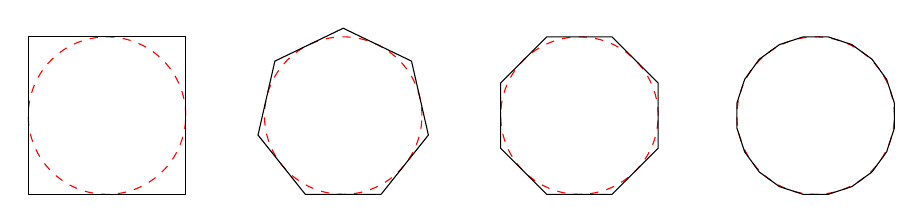
\begin{tikzpicture}
		\draw[red,dashed] (0,0) circle (1);
		\draw (0,0) \polygon{4}{1};
	
		\draw[red,dashed] (3,0) circle (1);
		\draw (3,0) \polygon{7}{1};

		\draw[red,dashed] (6,0) circle (1);
		\draw (6,0) \polygon{8}{1};

		\draw[red,dashed] (9,0) circle (1);
		\draw (9,0) \polygon{20}{1};

	\end{tikzpicture}
	\caption{(from left to right) Polygons with 4 sides, 7 sides, 8 sides and 100 sides used to approximate the circle drawn in red.}
	\label{fig:circle}
\end{figure}
\tiny{
\begin{verbatim}
\usepackage{tikz}
\usetikzlibrary{calc}
\newcommand{\polygon}[2]{%
  let \n{len} = {2*#2*tan(360/(2*#1))} in
 ++(0,-#2) ++(\n{len}/2,0) \foreach \x in {1,...,#1} { -- ++(\x*360/#1:\n{len})}}
...
	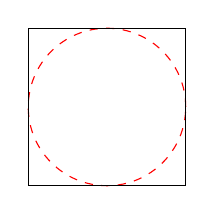
\begin{tikzpicture}
		\draw[red,dashed] (0,0) circle (1);
		\draw (0,0) \polygon{4}{1};
	\end{tikzpicture}
\end{verbatim}
}
\end{frame}


%------------------------------------------------------------------------------
\begin{frame}[fragile]{TikZ vector fields}
\begin{figure}
	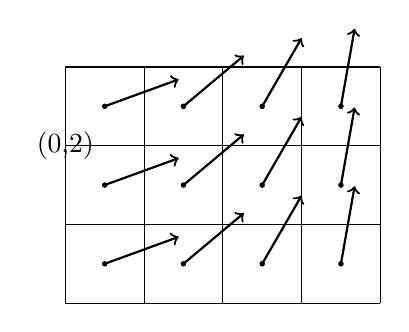
\begin{tikzpicture}
	\draw (0, 0) grid (4, 3);
	\foreach \x/\angle in {0.5/20, 1.5/40, 2.5/60, 3.5/80} {
	    \foreach \y in {0.5, 1.5, 2.5} {
    	    \fill (\x,\y) circle[radius=1pt];
        	\draw[->,thick]  (\x, \y) -- ++(\angle:1);
    	}
	}
	\node at (0,2) {(0,2)}; 
	\end{tikzpicture}
	\caption{You can plot vector fields as well.}
	\label{fig:vectors}
\end{figure}
\tiny{
\begin{verbatim}
\begin{figure}
	\begin{tikzpicture}
	\draw (0, 0) grid (4, 3); % draw a grid
	\foreach \x/\angle in {0.5/20, 1.5/40, 2.5/60, 3.5/80} { % loop over x and angle
	    \foreach \y in {0.5, 1.5, 2.5} { % loop over y
    	    \fill (\x,\y) circle[radius=1pt]; % draw circle at grid center
        	\draw[->,thick]  (\x, \y) -- ++(\angle:1); % draw line with arrowhead
    	}
	}
	\node[draw,text width=4cm] at (0,2) {(0,2)} % annotate the plot 
	\end{tikzpicture}
	\caption{You can plot vector fields as well.}
	\label{fig:vectors}
\end{figure}
\end{verbatim}
}
\end{frame}
%------------------------------------------------------------------------------
\begin{frame}{Useful links}
	\begin{itemize}
		\item \href{https://www.coga.tu-berlin.de/fileadmin/i26/download/AG_DiskAlg/FG_KombOptGraphAlg/kappmeier/How_to_TikZ_-_current.pdf}{How to TikZ}
		\item \href{https://en.wikibooks.org/wiki/LaTeX/Labels_and_Cross-referencing}{cross-referencing}
		\item \href{https://en.wikibooks.org/wiki/LaTeX/Mathematics}{Math symbols}
		\item \href{https://en.wikibooks.org/wiki/LaTeX/Mathematics}{Hyperlinks} (e.g. for \textit{mailto:})
		\item \href{mailto:bsulatex@cgiss.boisestate.edu}{bsulatex@cgiss.boisestate.edu}
	\end{itemize}	
\end{frame}
%------------------------------------------------------------------------------
\begin{frame}{Ackowledgments}

	A lot of the introductory material presented here was taken from Tobi Oetiker's \textit{The Not So Short Introduction to \latex} found 

	\href{https://tobi.oetiker.ch/lshort/lshort.pdf}{here}.

\end{frame}
%------------------------------------------------------------------------------
\begin{frame}{BSU thesis template}
\ldots
\end{frame}

\end{document}
